% Practice Test 13 — Texas Edition
% Questions: 30 (18 MC + 12 SA)
% Generated by scripts/generate_practice_tests.py

\begin{practiceQuestion}{1-3-q16}{mc}
\begin{questionText}
A map uses a scale where $1$ cm represents $25$ km. What is the constant of proportionality in km per cm?
\end{questionText}
\choiceA{$0.04$}
\choiceB{$1$}
\choiceC{$25$}
\choiceD{$250$}
\correctAnswer{C}
\explanation{$k = \frac{25 \text{ km}}{1 \text{ cm}} = 25$ km per cm.}
\end{practiceQuestion}

\begin{practiceQuestion}{1-6-q18}{mc}
\begin{questionText}
A painter can paint $3$ rooms in $7$ hours. At this rate, how many hours will it take to paint $9$ rooms?
\end{questionText}
\choiceA{$14$}
\choiceB{$18$}
\choiceC{$21$}
\choiceD{$24$}
\correctAnswer{C}
\explanation{$\frac{3}{7} = \frac{9}{h}$. Cross-multiply: $3h = 63$, so $h = 21$ hours.}
\end{practiceQuestion}

\begin{practiceQuestion}{2-1-q14}{mc}
\begin{questionText}
What is $150\%$ of $40$?
\end{questionText}
\choiceA{$20$}
\choiceB{$40$}
\choiceC{$50$}
\choiceD{$60$}
\correctAnswer{D}
\explanation{$150\% = 1.50$. Multiply: $1.50 \times 40 = 60$. A percent greater than $100\%$ gives a result greater than the whole.}
\end{practiceQuestion}

\begin{practiceQuestion}{2-3-q19}{sa}
\begin{questionText}
A puppy weighed $6$ pounds and now weighs $9$ pounds. What is the percent increase in weight?


\numberLine[1]{6}{10}
\end{questionText}
\correctAnswer{$50\%$}
\explanation{Change: $9 - 6 = 3$. Percent increase: $3 \div 6 = 0.50 = 50\%$.}
\end{practiceQuestion}

\begin{practiceQuestion}{2-6-q30}{gsa}
\begin{questionText}
The table below shows two loan options. Find the total cost (principal + interest) of each loan and determine how much more Loan B costs than Loan A.

\begin{center}
\begin{tabular}{|l|c|c|c|}
\hline
 & \textbf{Principal} & \textbf{Rate} & \textbf{Time} \\
\hline
Loan A & $\$5{,}000$ & $4\%$ & $3$ years \\
\hline
Loan B & $\$5{,}000$ & $7\%$ & $3$ years \\
\hline
\end{tabular}
\end{center}
\end{questionText}
\correctAnswer{Loan B costs $\$450$ more}
\explanation{Loan A interest: $5{,}000 \times 0.04 \times 3 = \$600$, total $= \$5{,}600$. Loan B interest: $5{,}000 \times 0.07 \times 3 = \$1{,}050$, total $= \$6{,}050$. Difference: $6{,}050 - 5{,}600 = \$450$.}
\end{practiceQuestion}

\begin{practiceQuestion}{2-8-q22}{sa}
\begin{questionText}
A $\$350$ purchase is paid with a credit card at $16\%$ annual interest. If paid after $1$ year, what is the total cost?
\end{questionText}
\correctAnswer{$\$406$}
\explanation{Interest $= 350 \times 0.16 = \$56$. Total $= 350 + 56 = \$406$.}
\end{practiceQuestion}

\begin{practiceQuestion}{2-9-q01}{mc}
\begin{questionText}
A budget shows income $= \$1{,}800$, fixed expenses $= \$1{,}000$, variable expenses $= \$500$. How much is left to save?
\end{questionText}
\choiceA{$\$200$}
\choiceB{$\$300$}
\choiceC{$\$500$}
\choiceD{$\$800$}
\correctAnswer{B}
\explanation{Savings $= 1{,}800 - 1{,}000 - 500 = \$300$.}
\end{practiceQuestion}

\begin{practiceQuestion}{2-10-q15}{mc}
\begin{questionText}
Why is compound interest sometimes called ``interest on interest''?
\end{questionText}
\choiceA{The bank charges interest twice}
\choiceB{Each year the interest is calculated on the total, including past interest}
\choiceC{You earn interest only if you don't withdraw}
\choiceD{The rate doubles each year}
\correctAnswer{B}
\explanation{With compound interest, each year's interest is added to the total, so the next year's interest is larger.}
\end{practiceQuestion}

\begin{practiceQuestion}{4-1-q21}{sa}
\begin{questionText}
A pool is being filled at a rate of $8$ gallons per minute. It already has $50$ gallons of water. Write an expression for the amount of water after $t$ minutes, then find the amount after $15$ minutes.
\end{questionText}
\correctAnswer{$8t + 50$; $170$ gallons}
\explanation{The expression is $8t + 50$. Substitute $t = 15$: $8(15) + 50 = 120 + 50 = 170$ gallons.}
\end{practiceQuestion}

\begin{practiceQuestion}{4-2-q26}{gmc}
\begin{questionText}
The algebra tiles below represent an expression. Which is the simplified form?

\begin{center}
\begin{tikzpicture}[scale=0.55]
  % Positive x-tiles
  \fill[funBlue!40] (0,0) rectangle (2,1);
  \draw[thick] (0,0) rectangle (2,1);
  \node at (1,0.5) {$x$};
  \fill[funBlue!40] (2.3,0) rectangle (4.3,1);
  \draw[thick] (2.3,0) rectangle (4.3,1);
  \node at (3.3,0.5) {$x$};
  \fill[funBlue!40] (4.6,0) rectangle (6.6,1);
  \draw[thick] (4.6,0) rectangle (6.6,1);
  \node at (5.6,0.5) {$x$};
  \fill[funBlue!40] (6.9,0) rectangle (8.9,1);
  \draw[thick] (6.9,0) rectangle (8.9,1);
  \node at (7.9,0.5) {$x$};
  \fill[funBlue!40] (9.2,0) rectangle (11.2,1);
  \draw[thick] (9.2,0) rectangle (11.2,1);
  \node at (10.2,0.5) {$x$};
  % Negative x-tiles
  \fill[funRed!40] (0,-1.5) rectangle (2,-0.5);
  \draw[thick] (0,-1.5) rectangle (2,-0.5);
  \node at (1,-1) {$-x$};
  \fill[funRed!40] (2.3,-1.5) rectangle (4.3,-0.5);
  \draw[thick] (2.3,-1.5) rectangle (4.3,-0.5);
  \node at (3.3,-1) {$-x$};
  % Positive unit tiles
  \fill[funGreen!40] (6,-1.5) rectangle (7,-0.5);
  \draw[thick] (6,-1.5) rectangle (7,-0.5);
  \node at (6.5,-1) {$1$};
  \fill[funGreen!40] (7.3,-1.5) rectangle (8.3,-0.5);
  \draw[thick] (7.3,-1.5) rectangle (8.3,-0.5);
  \node at (7.8,-1) {$1$};
  \fill[funGreen!40] (8.6,-1.5) rectangle (9.6,-0.5);
  \draw[thick] (8.6,-1.5) rectangle (9.6,-0.5);
  \node at (9.1,-1) {$1$};
  \fill[funGreen!40] (9.9,-1.5) rectangle (10.9,-0.5);
  \draw[thick] (9.9,-1.5) rectangle (10.9,-0.5);
  \node at (10.4,-1) {$1$};
\end{tikzpicture}
\end{center}
\end{questionText}
\choiceA{$5x + 4$}
\choiceB{$3x + 4$}
\choiceC{$7x + 4$}
\choiceD{$3x - 4$}
\correctAnswer{B}
\explanation{There are $5$ positive $x$-tiles and $2$ negative $x$-tiles: $5x + (-2x) = 3x$. There are $4$ positive unit tiles: $+4$. Simplified: $3x + 4$.}
\end{practiceQuestion}

\begin{practiceQuestion}{5-3-q06}{mc}
\begin{questionText}
Which equation is equivalent to $4(x + 5) = 36$?
\end{questionText}
\choiceA{$4x + 5 = 36$}
\choiceB{$4x + 20 = 36$}
\choiceC{$4x + 9 = 36$}
\choiceD{$x + 20 = 36$}
\correctAnswer{B}
\explanation{Distribute $4$: $4 \times x + 4 \times 5 = 4x + 20$. So the equation becomes $4x + 20 = 36$.}
\end{practiceQuestion}

\begin{practiceQuestion}{5-4-q20}{sa}
\begin{questionText}
Solve $0.75y + 2.25 = 8.25$.
\end{questionText}
\correctAnswer{$y = 8$}
\explanation{Subtract $2.25$: $0.75y = 6$. Divide by $0.75$: $y = 8$. Check: $0.75(8) + 2.25 = 6 + 2.25 = 8.25$ \checkmark.}
\end{practiceQuestion}

\begin{practiceQuestion}{5-5-q16}{mc}
\begin{questionText}
Solve $\dfrac{n}{5} - 2 > 4$.
\end{questionText}
\choiceA{$n > 10$}
\choiceB{$n > 30$}
\choiceC{$n > 1$}
\choiceD{$n < 30$}
\correctAnswer{B}
\explanation{Add $2$: $\frac{n}{5} > 6$. Multiply by $5$: $n > 30$.}
\end{practiceQuestion}

\begin{practiceQuestion}{5-6-q08}{mc}
\begin{questionText}
Solve $4x + 3 \leq 19$ and describe the graph.
\end{questionText}
\choiceA{Closed circle at $4$, shade left}
\choiceB{Open circle at $4$, shade left}
\choiceC{Closed circle at $4$, shade right}
\choiceD{Closed circle at $5.5$, shade left}
\correctAnswer{A}
\explanation{Subtract $3$: $4x \leq 16$. Divide by $4$: $x \leq 4$. Closed circle at $4$, shade left.}
\end{practiceQuestion}

\begin{practiceQuestion}{6-2-q23}{sa}
\begin{questionText}
A park is drawn at scale $1$ cm $= 50$ m. The park is $8$ cm wide on this drawing. If the new drawing must show the park as $4$ cm wide, what scale should the new drawing use?
\end{questionText}
\correctAnswer{$1$ cm $= 100$ m}
\explanation{Actual width: $8 \times 50 = 400$ m. New scale: $400 \div 4 = 100$ m per cm.}
\end{practiceQuestion}

\begin{practiceQuestion}{6-3-q12}{mc}
\begin{questionText}
Two angles of a triangle are $30°$ and $90°$. How many triangles can be drawn with these two angles and a hypotenuse of $10$ cm?
\end{questionText}
\choiceA{None}
\choiceB{Exactly one}
\choiceC{Exactly two}
\choiceD{Infinitely many}
\correctAnswer{B}
\explanation{The third angle is $180° - 30° - 90° = 60°$. With two angles and a specific side (AAS), exactly one triangle is determined.}
\end{practiceQuestion}

\begin{practiceQuestion}{6-4-q09}{mc}
\begin{questionText}
A triangle has angles $90°$, $45°$, and $45°$. Which statement is true?
\end{questionText}
\choiceA{Exactly one such triangle exists}
\choiceB{Many triangles with these angles exist, in different sizes}
\choiceC{No such triangle exists because two angles are equal}
\choiceD{No such triangle exists because the angles don't sum to $180°$}
\correctAnswer{B}
\explanation{$90 + 45 + 45 = 180°$ \checkmark. But AAA alone allows different sizes. Many $45$-$45$-$90$ triangles exist.}
\end{practiceQuestion}

\begin{practiceQuestion}{6-5-q14}{mc}
\begin{questionText}
Which cross-section is NOT possible from slicing a rectangular prism?
\end{questionText}
\choiceA{Rectangle}
\choiceB{Triangle}
\choiceC{Circle}
\choiceD{Pentagon}
\correctAnswer{C}
\explanation{A rectangular prism has flat faces and straight edges. Its cross-sections can be triangles, rectangles, pentagons, or hexagons, but never circles (since it has no curved surfaces).}
\end{practiceQuestion}

\begin{practiceQuestion}{6-8-q27}{gmc}
\begin{questionText}
The diagram shows two similar triangles. Find the missing side length $n$.

\begin{center}
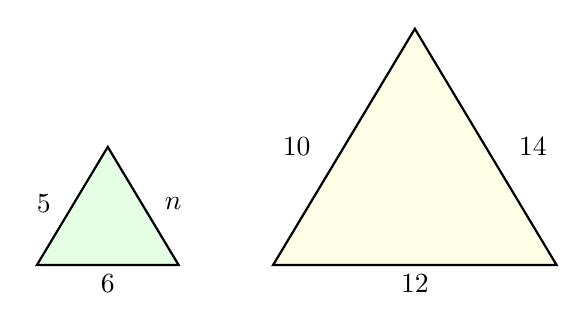
\begin{tikzpicture}[scale=0.6]
  % Small triangle
  \draw[thick,fill=green!10] (0,0) -- (3,0) -- (1.5,2.5) -- cycle;
  \node[below] at (1.5,0) {$6$};
  \node[left] at (0.5,1.3) {$5$};
  \node[right] at (2.5,1.3) {$n$};
  % Large triangle
  \draw[thick,fill=yellow!10] (5,0) -- (11,0) -- (8,5) -- cycle;
  \node[below] at (8,0) {$12$};
  \node[left] at (6,2.5) {$10$};
  \node[right] at (10,2.5) {$14$};
\end{tikzpicture}
\end{center}
\end{questionText}
\choiceA{$4$}
\choiceB{$7$}
\choiceC{$8$}
\choiceD{$9$}
\correctAnswer{B}
\explanation{Scale factor: $\frac{6}{12} = 0.5$ (or $\frac{5}{10} = 0.5$). $n = 14 \times 0.5 = 7$.}
\end{practiceQuestion}

\begin{practiceQuestion}{7-4-q08}{mc}
\begin{questionText}
A composite shape is made of a rectangle $7$ m by $4$ m with a semicircle of diameter $4$ m on one short side. What is the total area? Use $\pi \approx 3.14$.
\end{questionText}
\choiceA{$28$ m$^2$}
\choiceB{$34.28$ m$^2$}
\choiceC{$40.56$ m$^2$}
\choiceD{$53.12$ m$^2$}
\correctAnswer{B}
\explanation{Rectangle: $7 \times 4 = 28$ m$^2$. Semicircle: $\frac{1}{2} \times 3.14 \times 2^2 = \frac{1}{2} \times 3.14 \times 4 = 6.28$ m$^2$. Total: $28 + 6.28 = 34.28$ m$^2$.}
\end{practiceQuestion}

\begin{practiceQuestion}{7-5-q20}{sa}
\begin{questionText}
A cube has a side length of $7$ m. What is its surface area?
\end{questionText}
\correctAnswer{$294$ m$^2$}
\explanation{$SA = 6s^2 = 6 \times 49 = 294$ m$^2$.}
\end{practiceQuestion}

\begin{practiceQuestion}{7-6-q19}{sa}
\begin{questionText}
Find the volume of a rectangular prism with dimensions $9$ cm by $5$ cm by $4$ cm.
\end{questionText}
\correctAnswer{$180$ cm$^3$}
\explanation{$V = 9 \times 5 \times 4 = 180$ cm$^3$.}
\end{practiceQuestion}

\begin{practiceQuestion}{8-1-q29}{gsa}
\begin{questionText}
The bar graph shows the results of surveying a random sample of $60$ students about how they get to school.

\begin{center}
\begin{tikzpicture}[scale=0.65]
  \draw[thick,->] (0,0) -- (0,6) node[above]{\small Students};
  \draw[thick,->] (0,0) -- (7,0);
  \fill[funBlue!70] (0.5,0) rectangle (1.5,5);
  \fill[funGreen!70] (2.5,0) rectangle (3.5,3);
  \fill[funOrange!70] (4.5,0) rectangle (5.5,2);
  \node[below,font=\small] at (1,-0.1) {Bus};
  \node[below,font=\small] at (3,-0.1) {Walk};
  \node[below,font=\small] at (5,-0.1) {Car};
  \foreach \y in {1,...,5} {
    \draw (-0.1,\y) -- (0.1,\y);
    \node[left,font=\small] at (0,\y) {$\y\times6$};
  }
  \node[above,font=\small] at (1,5) {$30$};
  \node[above,font=\small] at (3,3) {$18$};
  \node[above,font=\small] at (5,2) {$12$};
\end{tikzpicture}
\end{center}

If the school has $900$ students, predict how many walk to school.
\end{questionText}
\correctAnswer{$270$}
\explanation{$\frac{18}{60} = 30\%$. Then $30\%$ of $900 = 270$.}
\end{practiceQuestion}

\begin{practiceQuestion}{8-2-q23}{sa}
\begin{questionText}
Explain why using a larger sample size generally leads to better predictions about a population.
\end{questionText}
\correctAnswer{A larger sample reduces the effect of random variation and better represents the population}
\explanation{Larger samples include more members of the population, so the sample statistics are closer to the true population values.}
\end{practiceQuestion}

\begin{practiceQuestion}{8-4-q15}{mc}
\begin{questionText}
Why is it important to use multiple measures (mean, median, range, IQR, MAD) when comparing two groups?
\end{questionText}
\choiceA{One measure tells the complete story}
\choiceB{Using more measures wastes time}
\choiceC{Different measures reveal different aspects of the data}
\choiceD{All measures always give the same conclusion}
\correctAnswer{C}
\explanation{Mean and median show center; range, IQR, and MAD show spread. Together they give a complete picture.}
\end{practiceQuestion}

\begin{practiceQuestion}{8-5-q20}{sa}
\begin{questionText}
Using the stem-and-leaf plot: Stem $7$: $0\;\;3\;\;5\;\;8$; Stem $8$: $1\;\;4\;\;6$; Stem $9$: $0\;\;5$. Find the median.
\end{questionText}
\correctAnswer{$81$}
\explanation{Data: $70, 73, 75, 78, 81, 84, 86, 90, 95$. There are $9$ values; the $5$th is $81$.}
\end{practiceQuestion}

\begin{practiceQuestion}{8-6-q24}{sa}
\begin{questionText}
Three categories in a circle graph have angles $150°$, $90°$, and $x°$. Find $x$.
\end{questionText}
\correctAnswer{$120°$}
\explanation{$150 + 90 + x = 360$, so $x = 360 - 240 = 120°$.}
\end{practiceQuestion}

\begin{practiceQuestion}{9-4-q18}{mc}
\begin{questionText}
Ben predicts that a coin will land on heads $50\%$ of the time. He flips the coin $20$ times and gets $14$ heads. What should he conclude?
\end{questionText}
\choiceA{The coin is definitely biased}
\choiceB{His model is exactly correct}
\choiceC{The result is somewhat different from the prediction, but $20$ trials is a small sample}
\choiceD{He should change his model to predict $70\%$ heads}
\correctAnswer{C}
\explanation{$\frac{14}{20} = 0.70$ vs. predicted $0.50$. With only $20$ trials, variation is expected. More trials would provide a better comparison.}
\end{practiceQuestion}

\begin{practiceQuestion}{9-6-q28}{gmc}
\begin{questionText}
The table below shows the sample space for spinning two spinners. Spinner 1 has sections $\{1, 2, 3\}$ and Spinner 2 has sections $\{A, B\}$. If each outcome is equally likely, what is the probability of getting an odd number and the letter B?

\begin{center}
\begin{tabular}{|c|c|c|}
\hline
 & \textbf{A} & \textbf{B} \\
\hline
\textbf{1} & $(1,A)$ & \cellcolor{funGreen!20}$(1,B)$ \\
\hline
\textbf{2} & $(2,A)$ & $(2,B)$ \\
\hline
\textbf{3} & $(3,A)$ & \cellcolor{funGreen!20}$(3,B)$ \\
\hline
\end{tabular}
\end{center}
\end{questionText}
\choiceA{$\frac{1}{6}$}
\choiceB{$\frac{2}{6}$}
\choiceC{$\frac{3}{6}$}
\choiceD{$\frac{4}{6}$}
\correctAnswer{B}
\explanation{Odd numbers: $1, 3$. Favorable outcomes: $(1,B)$ and $(3,B)$ — $2$ out of $6$. $P = \frac{2}{6} = \frac{1}{3}$.}
\end{practiceQuestion}

\begin{practiceQuestion}{9-7-q02}{mc}
\begin{questionText}
A coin flip is used to simulate an event with two equally likely outcomes. Which real-world event could it model?
\end{questionText}
\choiceA{The probability of rain ($30\%$ chance)}
\choiceB{Whether a baby is a boy or girl (approximately $50\%$ each)}
\choiceC{Rolling a $6$ on a die}
\choiceD{Drawing a heart from a deck of cards}
\correctAnswer{B}
\explanation{A coin has two equally likely outcomes ($50\%$ each), which matches the approximately $50/50$ chance of a baby being a boy or girl.}
\end{practiceQuestion}
